\documentclass[conference]{IEEEtran}
\IEEEoverridecommandlockouts
% The preceding line is only needed to identify funding in the first footnote. If that is unneeded, please comment it out.
\usepackage{cite}
\usepackage{amsmath,amssymb,amsfonts}
\usepackage{algorithmic}
\usepackage{graphicx}
\usepackage{textcomp}
\usepackage{xcolor}
\usepackage{url}

% added
\usepackage{microtype}
\usepackage{multirow}
\usepackage{multicol}
\newtheorem{example}{Example}
\usepackage{amsmath}
\newcommand{\secref}[1]{Section \ref{#1}}
\newcommand{\figref}[1]{Figure \ref{#1}}
\newcommand{\eqnref}[1]{Eq. (\ref{#1})}
\newcommand{\tabref}[1]{Table \ref{#1}}
\newcommand{\exref}[1]{Example \ref{#1}}
\newcommand{\cut}[1]{}
\newcommand{\KZ}[1]{\textcolor{blue}{Kenny: #1}}
\newcommand\BibTeX{B\textsc{ib}\TeX}
\newcommand{\sgn}{\text{sgn}}

\def\BibTeX{{\rm B\kern-.05em{\sc i\kern-.025em b}\kern-.08em
    T\kern-.1667em\lower.7ex\hbox{E}\kern-.125emX}}
\begin{document}

\title{ICQ: Visualizing Statistical Biases in Discriminative Text Inference Tasks and Models}
%{\footnotesize \textsuperscript{*}Note: Sub-titles are not captured in Xplore and
%should not be used}
%\thanks{Identify applicable funding agency here. If none, delete this.}

\author{\IEEEauthorblockN{Shanshan Huang}
\IEEEauthorblockA{\textit{Shanghai Jiao Tong University}\\
Shanghai, China\\
huangss\_33@sjtu.edu.cn}
\and
\IEEEauthorblockN{Kenny Q. Zhu}
\IEEEauthorblockA{\textit{Shanghai Jiao Tong University}\\
Shanghai, China\\
kzhu@cs.sjtu.edu.cn}
}


\maketitle
\begin{abstract}
Recent work has identified that many natural language understanding and 
reasoning datasets contain statistical cues that
may be taken advantaged of by sophisticated models and hence overestimate the 
capability of these models. 
%However, none of the work has been able to
%easily pinpoint what these cues are. 
%Inspired by black-box test in software engineering, 
Some human-designed stress tests have been proposed to mitigate this problem
but they are expensive to create and do not generalize to arbitrary models. 
We propose a light-weight visualization framework, ICQ, 
which automatically identifies possible biases
in any text inference multiple-choice datasets without creating any additonal
test cases, and further evaluates
the robustness of any black-box models targeting the datasets. 
\end{abstract}

%\IEEEraisesectionheading{
% %\IEEEraisesectionheading{
% %\IEEEraisesectionheading{
% \input{intro}
\section{Introduction}\label{sec:intro}
 %}
% \section{Introduction}\label{sec:intro}

% \begin{enumerate}
% \item Motivation: application scenarios (with 1-2 running examples);
% \item Characteristics of the data sources and their challenges;
% \item Briefly introduce previous approaches to extract information 
% from images including setting the document zone, and their limitations.
% \item General flow of our approach (may give a diagram here)
% \end{enumerate}
% scenary

Due to ever evolving hardware and software, many medical images
such as electro-cardio graphs (ECGs), X-ray or ultrasound images  
are directly printed and stored in hard copy formats. 
% \KZ{Insert 4 example images here.}
%Examples are shown in \figref{fig:medicalImages}. 
% These images often contain a mix of graphics and text, which
% include parameter settings of the hardware, test measurements or simple
% diagnosis. 
These images often contain a mix of graphics and text, which 
include technical settings of the hardware used, test measurements or simple diagnoses.
Recently, there has been a growing demand for digitizing such 
medical information from paper media sources, especially legacy ones, or patients who want to keep track of these documents by themselves digitally. 
Apart from scanning the graphics into a digital format, extracting 
the semi-structured textual information is also an important part of
building electronic medical records for patients. 

%\begin{figure}[!htb]
%\centering
%\subfloat[ECG]{
%\label{fig:medicalimage:ecg}
%\epsfig{file=figure/17_ori.eps, width=0.4\columnwidth}
%}
%% \hfill
%\subfloat[MRI]{
%	\label{fig:medicalimage:mrt}
%	\epsfig{file=figure/MRI.eps, width=0.4\columnwidth}
%}
%\\
%\subfloat[X-RAY]{
%\label{fig:medicalimage:xray}
%\epsfig{file=figure/X-RAY.eps, width=0.4\columnwidth}
%}
%%\hfill
%\subfloat[EEG]{
%\label{fig:medicalimage:eeg}
%\epsfig{file=figure/EEG.eps, width=0.4\columnwidth}
%}
%\caption{Examples of Medical Images}
%\label{fig:medicalImages}
%\end{figure}

Optical character recognition (OCR)  \cite{mori1992historical,smith2007overview} is 
a traditional technique used to turn images of printed text into machine encoded
text. It is well researched and performs well on plain text 
documents such as novels and reports, for a variety of languages. 
%For example, Tesseract, which is one of 
%the most popular open source multilingual recognizers, logs an error 
%rate of 3.72\% for English words and 3.77\% for simplified 
%Chinese characters\cite{smith2009adapting}. 
%Google Books \cite{googlebooks} and Gutenberg \cite{gutenberg} are
%projects which have scanned a large number of paper books into text for free and open
%access. These projects made exclusive use of OCR for this conversion and 
%achieved high accuracy \cite{vincent2007google} \cite{lebert2008project}. 
% 99\% for Gutenberg project \cite{lebert2008project}. 
% \KZ{Give the accuracy of google and gutenberg if available.}


\begin{figure}[th]
\centering
\epsfig{file=figure/17_b.eps, width=0.8\columnwidth}
\caption{An ECG image with text area (red circle) of interest.}
\label{fig:ecgexample2}
\end{figure}

For a semi-structured medical image, such as 
\figref{fig:ecgexample2}, we would like to extract the attribute-value 
pairs (e.g., {\em Vent. rate = 63 bpm}) and possibly other values such as
date ({\em 18-Nov-2010}) and time ({\em 9:13:02}) since those values endow us with lots of information about the patient. 
Existing OCR software cannot extract such structured information in a straightforward 
fashion, 
but instead it produces rather convoluted results from the whole image, 
similar to those in \figref{fig:ocrre}, which was produced by Tesseract, 
a popular multi-lingual recognizers. 
% \KZ{Maybe include the x-y coordinate info in the output as well?}  

\begin{figure}[th]
\centering
\scriptsize
\begin{verbatim}
<p class="ocr_par" title="box 263 33 444 119">
   <span class="ocr_l" title="box 264 33 336 45">
       <span class="ocrx_w" title="box 264 33 299 45">Vcnt.</span> 
       <span class="ocrx_w" title="box 308 34 336 45">rule</span> 
   </span>
   <span class='ocr_l'>
       <span class="ocrx_w" title="box 264 51 283 64">PR</span> 
       <span class="ocrx_w" title="box 291 51 346 64">Interval</span> 
       <span class="ocrx_w" title="box 389 52 411 64">140</span> 
       <span class="ocrx_w" title="box 420 55 439 64">ms</span> 
   </span>
   ...
   </span>
</p>
<p class="ocr_p" dir="ltr">
   <span class="ocr_l">
       <span class="ocrx_w" title="box 396 33 411 45">53</span> 
       <span class="ocrx_w" title="box 420 33 449 48">bpm</span> 
   </span>
</p>
\end{verbatim}
\caption{Snippet OCR results in XML, input to our framework.}
\label{fig:ocrre}
\end{figure}


%\input{xmlre1}

%However, OCR alone does not work well on semi-structured text and hence
%can't be directly used for information extraction from the aforementioned
%medical images. \KZ{Give the reason here, perhaps because OCR models are
%largely Markov based? So semi-structured data breaks the flow of text.}
%When a medical image is input to an ordinary OCR software, the spatial 
%information of the text components is often lost or mixed with noises
%and errors.
%%The reason is OCR converts the whole images into text data, in which 
%%useful information often mix with noises and errors. 
%In this paper, we would like to extract the attribute-value pairs
%and possibly other values from \figref{fig:ecgexample1} 
%and \figref{fig:ecgexample2}. 
%% or medical ultrasonography report. 
%Such images contain lots of non-textual information or noises.

% example & ref
%\begin{figure}[ht]
%\centering
%\epsfig{file=figure/46.eps, width=0.8\columnwidth}
%\caption{ECG Images From Printer1}
%\label{fig:ecgexample1}
%\end{figure}

% \begin{figure}[ht]
% \centering
% \subfloat[Printer1]{
% \label{fig:ecgexample:a}
% \epsfig{file=figure/46.eps, width=0.48\columnwidth}
% }
% \hfill
% \subfloat[Printer2]{
% \label{fig:ecgexample:b}
% \epsfig{file=figure/17.eps, width=0.48\columnwidth}
% }
% \caption{ECG images from two different printers}
% \label{fig:ecgexample}
% \end{figure}

Also, errors in the OCR text \cite{darwish2007error,taghva1996evaluation} will greatly affect the effectiveness 
of other related tasks. Much work has been done to improve the performance of the OCR\cite{kolak2003generative,cesarini1998informys}. However, there are still a number of significant challenges involved in extracting the information from medical images or OCR results in XML form. 

% First, medical images differ from pure text document in that them have 
% layout information. 
First, medical images differ from pure text documents in that 
they contain layout information.
Although most current OCR engines attempt to reproduce the physical 
layout of the text units, 
%(along with X-Y coordinates) and store them 
%in a special format such as XML 
% (\KZ{Better in the previous example})
such spatial
information is approximate and sometimes inaccurate, which is why neighboring
text blocks in \figref{fig:ecgexample2}, such as ``Vent. Rate'' and
``63 bpm'' were not automatically combined into the same XML block, but were 
rather far apart (shown in two different ``classes'') in \figref{fig:ocrre} made by OCR softwares. 
%Even for images produced by the same ECG printer, 
%the XML results can still be very different as 
The spatial layout is sensitive to many factors, such as accidental spots 
on the prints, color and contrast, or the angle of the camera. 
%In this case, solutions for other application domains, for example, the web, 
%are not well suited for information extraction from printed documents \cite{bartoli2014semisupervised}. With such inaccurate
%layout information produced by OCR,
%it is not easy to write a simple wrapper program to extract useful
%data from images, even if the images come from the same printer. 

%Writing a wrapper for each
%individual image would be tedious and counter-productive. Therefore,
%a mechanism that makes use of the spatial locality of the 
%text units in the image and 
%accommodates slight variations in the spatial layout would make the extraction
%more accurate and fault-tolerant.

%For example, \figref{fig:ocrre} is the simplified OCR results for the ECGs in 
%\figref{fig:ecgexample1} and \figref{fig:ecgexample2}. The results are in the XML format and have attritube named {\em class} 
%for layout information. Although these two images share similar format. 
%OCR engine generates different results in that it splits elements that 
%should be in the same line into two lines in the second example. 
%XML is sensitive to the layout results so it's hard to tolerate 
%all the layout results. 
%
% example check the term
% layout of ocr results can be restore, so why OCR engine don't restore the results 
% using the similar methods as we do?
% or the way we handle the layout problem is quite simple

% Delete for TIP
% Second, exiting OCR engines make heavy use of Markov properties such as n-grams
% since they primarily target the transformation of large body of text 
% \cite{kolak2003generative}. 
% % \KZ{Needs some refs here.}
% Unfortunately, the semi-structured texts in medical images are often 
% short and not even written in complete sentences, thus breaking Markov assumption. To make
% matters worse, medical images contain scientific language, which may be
% very different from the training corpora of these OCR engines.
% This explains why we see errors like ``Vcnt'' and ``rule'' 
% in \figref{fig:ocrre}. 
% %can't guarantee a perfect performance, which means 
% %there are errors and noises in the OCR results.
% %Many of them due to the fact that the data are no longer long, continous
% %sentences, thus breaking the Markov assumption made by many OCR algorithms. 
% %In \figref{fig:ocrresub:b}, ``Vent." is misrecognized as ``Vcnt.". 
% Without sufficient contextual information, OCR may also misrecognize a 
% digit as an alphabetic character, or as another similar digit. 
% Furthermore, the mix of text with images and formatting
% lines often confuses the OCR engine, which is more biased toward full
% text images.
% Exact pattern matching, as used in
% traditional information extraction, doesn't work with such noisy OCR output
% as it doesn't tolerate noises or errors in text. 
% %It's hard to autocorrect these errors 
% %because image quality is the most important affecting factor. 
% %The text we are processing can be full of no meaning words or 
% %strange numbers. 
% A fuzzy matching strategy is more desirable in this case. 
% % example, what are the traditional IEs

Second, there are many types of medical images, resulting from a variety of
medical tests. Different equipments for the same test can produce vastly 
different images. Writing individual extraction wrappers 
for the OCR outputs of all these formats is tedious and inefficient, 
and difficult for non-programmers.
%not to mention that there are significant programming barriers for 
%writing these wrappers, especially for the medical professionals who are the
%end users of these extraction results. 
%A more user-friendly approach enabling users to specify such extraction requirements would be preferred. 
%There are various kinds of medical images, such as electrocardiograph report, 
%medical ultrasonography report, etc. 
%However the basic measures for each type of medical test (e.g., ECG), 
%are very similar from machine to machine. Only the layouts are 
%different. 
% example medical images

Finally, most off-the-shelf OCR programs are pre-trained with specific 
recognition models, which may not be suitable for the extraction of 
%medical images.
%Furthermore, changes in imaging equipment technology over time may produce 
%different formats, layout, or terminology, rendering existing OCR models 
%obsolete. 
Re-training the models requires a large amount of labeled data, which may
not be available. 
%Incremental training as more labeled data arrives
%is currently not supported by any OCR product.    

%There have been some limited attempts to address some of the above challenges. 
%One solution is a plugin of an OCR program that allows the user to specify 
%target zones of interest in the image to be extracted. The zones specified for
%one image can be applied to images with slight variations by adjusting against
%a fixed reference point that is supposed to exist in all these images.
%% \KZ{I think the problem is not so much with the zones, because we also
%% have zones, but rather with the reference point.}
%% \JY{}
%% example products
%% http://www.square-9.com/automated-data-extraction-optical-character-recognition
%The problem with this solution is its high reliance on the OCR zones  
%established by the user. The performance of the results is affected by the 
%accuracy of the zones. If the zones are too big, the results will be full of 
%noise. If the zones are too small, results will miss something. 
%
%Another solution involves using the page layout analysis technique. The page layout 
%analysis technique is used to determine where the text 
%resides on a page \cite{o1993document}, 
%% \KZ{This page layout analysis approach is not clearly described. I don't understand after reading this paragraph.}
%% By using page layout analysis technique, the hierarchy of physical components 
%% can be generated and to match with the hierarchy of logical components, which 
%% is predefined. 
%this includes identifying and categorizing the 
%regions of interest in the scanned image of a text document. 
%Typically, the first step is to segment text zones from 
%non-textual zones and arrange them in their original order. 
%Then in order to analyze the logical roles of the text zones 
%(titles, captions, footnotes, etc.), logical layout analysis 
%is used for labeling the semantics of the text zones.
%Generally, page layout analysis is used for documents. The problem with applying 
%such a technique on medical images is that it creates so much noises 
%that performance is ultimately affected. 
%For medical imaging reports like ECG, useful information is often 
%found in the small components of the image, while most of the images are 
%read as noises. 
% check paper and more description, weakness, ref

%In this paper, 
%we propose a spatial data description language, which borrows its syntax from
%PADS \cite{fisher+:pads}, an ad hoc data processing language, 
%for describing semi-structured data in medical images. 
%% ref
%We call this language OCR description language, or ODL. 
%ODL is designed for extracting and parsing semi-structured text data 
%from images. We believe that  information extraction from those data in ODL form may be much easier than extracting information from rough data or data in XML form, which means that our preprocessing part proves to be necessary.
%%An example ODL description for the image in 
%%\figref{fig:ecgexample2} is shown in 
%%\figref{fig:description}. \KZ{Make this description two column, and give
%%some brief explanation of this description here.} 
%%The parsing result of this description is shown
%%in \figref{fig:parsing result}. \KZ{Give some explanation of the results,
%%otherwise don't show the result here. E.g., you need to explain what F, E, etc.
%%mean. You want to say that even though rate has been recognized as rule,
%%the bpm value was still extracted (but still wrong!).}
%% \KZ{I removed the preprocessing part, cos it's not important. Talk about it in
%% discussion sec.}
%%The our approach starts by preprocessing the images for text results.
%To use this framework, the user first describes the components in the image
%that he or she is interested in extracting. This includes constant strings
%and variables of different data types.   
%ODL allows the user to specify the approximate spatial layout and constraints on
%the data, e.g., integers within 
%a certain range, real numbers with certain decimal points, etc. 
%%This information is then as the key component in our fuzzy matching strategy. 
%The system then automatically generates a parser for these medical images.
%This parser uses the output XML from OCR with spatial information as an input, 
%and outputs a data structure with values extracted for each variables
%in the description, unless there is an unrecoverable error during the parsing process.
%In addition, approximate layout information and constraints are used in parsing process 
%to tolerate noises and small format variations in the input images. 
%%Specifically, this method could be called fuzzy matching, meaning that more candidates could be saved after the parsing process.  It's obvious that we may have a higher probability to obtain the accurate result if more candidates are kept so that fuzzy match should be used properly in our system.
%%An autogenerated parser based on the ODL description can release us from 
%%repetitive work. In this way, we turn the task of writing complex parsers 
%%into describing information on images.
%
%
%When users process many images of the same format, the system 
%automatically discovers parsing errors given the current model and 
%prompts the user to manually correct some of the frequent and prominent
%errors, which effectively serves as an online labeling function. 
%These incrementally labeled data are then used to update the parsing model. 


%It should be emphasized that the incremental learning model is very important in our whole system. Incremental learning is a machine learning paradigm where the learning process takes place whenever we have new examples or data added to our baisc data set, leading to a most striking difference between incremental learning and traditional machine learning: it does not assume the availability of a sufficient training set before the learning process. What incremental learning in our system is really impressive: it does not require a relatively good and stable training set at first time. In fact, it could improve the parsing result with even relatively rough training sets at first by absorbing new data or corrective information as time passes in dynamic systems. Besides, the process would be very effective when there are some new images coming in since training process would not learn from scratch, which might waste time and computation resource.

%At last, we propose an incrementally human correction framwork which can 
%make the best use of human correction to handle the misrecognition problem. 
% Base on our experiments on about 500 real life ECG images, 
% our approach achieves p1 and p2 after p3 times human correction. 
% experimental results

% \begin{figure}[h]
% \begin{lstlisting}
% Oenum str_month_t{
% 	"Jan", "Feb", "Mar", "Apr",
% 	"May", "Jun", "Jul", "Aug",
% 	"Sept", "Oct", "Nov", "Dec"
% };

% Ounion month_t{
% 	Oint(1,12)	num;
% 	str_month_t	str;
% };

% Ostruct time_t{
% 	Oint(1,31)	day;
% 	"-";
% 	month_t	month;
% 	"-";
% 	Oint	year;
% };

% Ostruct triple_t{
% 	"Vent.";
% 	hskip(\s)	skip1;
% 	"rate";
% 	Oint x;
% 	"bpm";
% 	vskip(\n)	skip2;
% };

% Oscource Ostruct entry_t{
% 	time_t(<-,-,-,0.3l>) t;
% 	triple_t(<0.1w,-,0.5w,->) d;
% };
% \end{lstlisting}
% \caption{Description}\label{fig:description}
% \end{figure}


In order to solve above problems, We design a system which makes three main contributions:
\begin{enumerate}
\item Based on some previous work on data description language \cite{lamport1986document,taft1999post,fisher+:pads},we design a new declarative spatial data description language called \textit{OCR description language}, or ODL,
which allows users to specify spatial and data constraints in medical 
images(\secref{sec:syntax});
\item We propose a noise-tolerant parser which takes OCR results
the ODL description as input and outputs a data structure with values 
extracted for each variables in the description (\secref{sec:semantics});
\item We propose an incremental manual correction 
framework\cite{von2008recaptcha,zhu2012learnpads++}, which 
takes advantage of user corrections  and improves the productivity
significantly (\secref{sec:correction}).
%To be more specific, the framework improves the traditional machine learning methods by using a incremental learning process to avoid starting from scratch when we are trying to apply human corrections in the system. That means the framework would be more effective than most corrective systems.
\end{enumerate}


\section{Introduction}\label{sec:intro}
 %}
% \section{Introduction}\label{sec:intro}

% \begin{enumerate}
% \item Motivation: application scenarios (with 1-2 running examples);
% \item Characteristics of the data sources and their challenges;
% \item Briefly introduce previous approaches to extract information 
% from images including setting the document zone, and their limitations.
% \item General flow of our approach (may give a diagram here)
% \end{enumerate}
% scenary

Due to ever evolving hardware and software, many medical images
such as electro-cardio graphs (ECGs), X-ray or ultrasound images  
are directly printed and stored in hard copy formats. 
% \KZ{Insert 4 example images here.}
%Examples are shown in \figref{fig:medicalImages}. 
% These images often contain a mix of graphics and text, which
% include parameter settings of the hardware, test measurements or simple
% diagnosis. 
These images often contain a mix of graphics and text, which 
include technical settings of the hardware used, test measurements or simple diagnoses.
Recently, there has been a growing demand for digitizing such 
medical information from paper media sources, especially legacy ones, or patients who want to keep track of these documents by themselves digitally. 
Apart from scanning the graphics into a digital format, extracting 
the semi-structured textual information is also an important part of
building electronic medical records for patients. 

%\begin{figure}[!htb]
%\centering
%\subfloat[ECG]{
%\label{fig:medicalimage:ecg}
%\epsfig{file=figure/17_ori.eps, width=0.4\columnwidth}
%}
%% \hfill
%\subfloat[MRI]{
%	\label{fig:medicalimage:mrt}
%	\epsfig{file=figure/MRI.eps, width=0.4\columnwidth}
%}
%\\
%\subfloat[X-RAY]{
%\label{fig:medicalimage:xray}
%\epsfig{file=figure/X-RAY.eps, width=0.4\columnwidth}
%}
%%\hfill
%\subfloat[EEG]{
%\label{fig:medicalimage:eeg}
%\epsfig{file=figure/EEG.eps, width=0.4\columnwidth}
%}
%\caption{Examples of Medical Images}
%\label{fig:medicalImages}
%\end{figure}

Optical character recognition (OCR)  \cite{mori1992historical,smith2007overview} is 
a traditional technique used to turn images of printed text into machine encoded
text. It is well researched and performs well on plain text 
documents such as novels and reports, for a variety of languages. 
%For example, Tesseract, which is one of 
%the most popular open source multilingual recognizers, logs an error 
%rate of 3.72\% for English words and 3.77\% for simplified 
%Chinese characters\cite{smith2009adapting}. 
%Google Books \cite{googlebooks} and Gutenberg \cite{gutenberg} are
%projects which have scanned a large number of paper books into text for free and open
%access. These projects made exclusive use of OCR for this conversion and 
%achieved high accuracy \cite{vincent2007google} \cite{lebert2008project}. 
% 99\% for Gutenberg project \cite{lebert2008project}. 
% \KZ{Give the accuracy of google and gutenberg if available.}


\begin{figure}[th]
\centering
\epsfig{file=figure/17_b.eps, width=0.8\columnwidth}
\caption{An ECG image with text area (red circle) of interest.}
\label{fig:ecgexample2}
\end{figure}

For a semi-structured medical image, such as 
\figref{fig:ecgexample2}, we would like to extract the attribute-value 
pairs (e.g., {\em Vent. rate = 63 bpm}) and possibly other values such as
date ({\em 18-Nov-2010}) and time ({\em 9:13:02}) since those values endow us with lots of information about the patient. 
Existing OCR software cannot extract such structured information in a straightforward 
fashion, 
but instead it produces rather convoluted results from the whole image, 
similar to those in \figref{fig:ocrre}, which was produced by Tesseract, 
a popular multi-lingual recognizers. 
% \KZ{Maybe include the x-y coordinate info in the output as well?}  

\begin{figure}[th]
\centering
\scriptsize
\begin{verbatim}
<p class="ocr_par" title="box 263 33 444 119">
   <span class="ocr_l" title="box 264 33 336 45">
       <span class="ocrx_w" title="box 264 33 299 45">Vcnt.</span> 
       <span class="ocrx_w" title="box 308 34 336 45">rule</span> 
   </span>
   <span class='ocr_l'>
       <span class="ocrx_w" title="box 264 51 283 64">PR</span> 
       <span class="ocrx_w" title="box 291 51 346 64">Interval</span> 
       <span class="ocrx_w" title="box 389 52 411 64">140</span> 
       <span class="ocrx_w" title="box 420 55 439 64">ms</span> 
   </span>
   ...
   </span>
</p>
<p class="ocr_p" dir="ltr">
   <span class="ocr_l">
       <span class="ocrx_w" title="box 396 33 411 45">53</span> 
       <span class="ocrx_w" title="box 420 33 449 48">bpm</span> 
   </span>
</p>
\end{verbatim}
\caption{Snippet OCR results in XML, input to our framework.}
\label{fig:ocrre}
\end{figure}


%% \begin{figure}[ht]
% \centering
% \subfigure[]{
% \label{fig:subfig:a}
% \begin{minipage}[b]{0.2\textwidth}
%\newsavebox{\firstlisting}
%\begin{lrbox}{\firstlisting}% Store first listing
%\begin{lstlisting}
%<p class='ocr_par' dir='ltr'>
%   <span class='ocr_line' id='line_2'>
%       <span class='ocrx_word' id='word_6'>Vent.</span>
%       <span class='ocrx_word' id='word_7'>rate</span>
%       <span class='ocrx_word' id='word_8'>65</span>
%       <span class='ocrx_word' id='word_9'>bpm</span>
%   </span>
%   <span class='ocr_line' id='line_3'>
%       <span class='ocrx_word' id='word_14'>PR</span>
%       <span class='ocrx_word' id='word_15'>interval</span>
%       <span class='ocrx_word' id='word_16'>162</span>
%       <span class='ocrx_word' id='word_17'>ms</span>
%   </span>
%    ...
%</p>
%\end{lstlisting}
%\end{lrbox}
% \end{minipage}
% }
% \hspace[1in]
% \subfigure[]{
% % \label{fig:subfig:b}
% % \begin{minipage}[b]{0.2\textwidth}
\newsavebox{\secondlisting}
\begin{lrbox}{\secondlisting}
% \tiny
\begin{lstlisting}[basicstyle=\tiny,]
<p class="ocr_par" title="box 263 33 444 119">
   <span class="ocr_l" title="box 264 33 336 45">
       <span class="ocrx_w" title="box 264 33 299 45">Vcnt.</span>
       <span class="ocrx_w" title="box 308 34 336 45">rule</span>
   </span>
   <span class='ocr_l'>
       <span class="ocrx_w" title="box 264 51 283 64">PR</span>
       <span class="ocrx_w" title="box 291 51 346 64">Interval</span>
       <span class="ocrx_w" title="box 389 52 411 64">140</span>
       <span class="ocrx_w" title="box 420 55 439 64">ms</span>
   </span>
   ...
   </span>
</p>
<p class="ocr_p" dir="ltr">
   <span class="ocr_l">
       <span class="ocrx_w" title="box 396 33 411 45">53</span>
       <span class="ocrx_w" title="box 420 33 449 48">bpm</span>
   </span>
</p>
\end{lstlisting}
\end{lrbox}
% % \end{minipage}
% }

% \KZ{\figref{fig:ocrre} is output from what software? Tesseract?}
\begin{figure*}[th]
%\subfloat[Image From Printer1]{
%\label{fig:ocrresub:a}
%\scalebox{0.8}{\usebox{\firstlisting}}}
%\hfill
%\subfloat[Image From Printer2]{
\scalebox{1.6}{\usebox{\secondlisting}}
% \label{fig:ocrre}
\caption{A fragment of raw OCR results for ECG with layout information.}
%\caption{Simplified OCR Results in XML for an ECG with Layout Information}
%\label{fig:ocrresub:b}
\label{fig:running-xml}
\end{figure*}

% \lipsum[2]


%However, OCR alone does not work well on semi-structured text and hence
%can't be directly used for information extraction from the aforementioned
%medical images. \KZ{Give the reason here, perhaps because OCR models are
%largely Markov based? So semi-structured data breaks the flow of text.}
%When a medical image is input to an ordinary OCR software, the spatial 
%information of the text components is often lost or mixed with noises
%and errors.
%%The reason is OCR converts the whole images into text data, in which 
%%useful information often mix with noises and errors. 
%In this paper, we would like to extract the attribute-value pairs
%and possibly other values from \figref{fig:ecgexample1} 
%and \figref{fig:ecgexample2}. 
%% or medical ultrasonography report. 
%Such images contain lots of non-textual information or noises.

% example & ref
%\begin{figure}[ht]
%\centering
%\epsfig{file=figure/46.eps, width=0.8\columnwidth}
%\caption{ECG Images From Printer1}
%\label{fig:ecgexample1}
%\end{figure}

% \begin{figure}[ht]
% \centering
% \subfloat[Printer1]{
% \label{fig:ecgexample:a}
% \epsfig{file=figure/46.eps, width=0.48\columnwidth}
% }
% \hfill
% \subfloat[Printer2]{
% \label{fig:ecgexample:b}
% \epsfig{file=figure/17.eps, width=0.48\columnwidth}
% }
% \caption{ECG images from two different printers}
% \label{fig:ecgexample}
% \end{figure}

Also, errors in the OCR text \cite{darwish2007error,taghva1996evaluation} will greatly affect the effectiveness 
of other related tasks. Much work has been done to improve the performance of the OCR\cite{kolak2003generative,cesarini1998informys}. However, there are still a number of significant challenges involved in extracting the information from medical images or OCR results in XML form. 

% First, medical images differ from pure text document in that them have 
% layout information. 
First, medical images differ from pure text documents in that 
they contain layout information.
Although most current OCR engines attempt to reproduce the physical 
layout of the text units, 
%(along with X-Y coordinates) and store them 
%in a special format such as XML 
% (\KZ{Better in the previous example})
such spatial
information is approximate and sometimes inaccurate, which is why neighboring
text blocks in \figref{fig:ecgexample2}, such as ``Vent. Rate'' and
``63 bpm'' were not automatically combined into the same XML block, but were 
rather far apart (shown in two different ``classes'') in \figref{fig:ocrre} made by OCR softwares. 
%Even for images produced by the same ECG printer, 
%the XML results can still be very different as 
The spatial layout is sensitive to many factors, such as accidental spots 
on the prints, color and contrast, or the angle of the camera. 
%In this case, solutions for other application domains, for example, the web, 
%are not well suited for information extraction from printed documents \cite{bartoli2014semisupervised}. With such inaccurate
%layout information produced by OCR,
%it is not easy to write a simple wrapper program to extract useful
%data from images, even if the images come from the same printer. 

%Writing a wrapper for each
%individual image would be tedious and counter-productive. Therefore,
%a mechanism that makes use of the spatial locality of the 
%text units in the image and 
%accommodates slight variations in the spatial layout would make the extraction
%more accurate and fault-tolerant.

%For example, \figref{fig:ocrre} is the simplified OCR results for the ECGs in 
%\figref{fig:ecgexample1} and \figref{fig:ecgexample2}. The results are in the XML format and have attritube named {\em class} 
%for layout information. Although these two images share similar format. 
%OCR engine generates different results in that it splits elements that 
%should be in the same line into two lines in the second example. 
%XML is sensitive to the layout results so it's hard to tolerate 
%all the layout results. 
%
% example check the term
% layout of ocr results can be restore, so why OCR engine don't restore the results 
% using the similar methods as we do?
% or the way we handle the layout problem is quite simple

% Delete for TIP
% Second, exiting OCR engines make heavy use of Markov properties such as n-grams
% since they primarily target the transformation of large body of text 
% \cite{kolak2003generative}. 
% % \KZ{Needs some refs here.}
% Unfortunately, the semi-structured texts in medical images are often 
% short and not even written in complete sentences, thus breaking Markov assumption. To make
% matters worse, medical images contain scientific language, which may be
% very different from the training corpora of these OCR engines.
% This explains why we see errors like ``Vcnt'' and ``rule'' 
% in \figref{fig:ocrre}. 
% %can't guarantee a perfect performance, which means 
% %there are errors and noises in the OCR results.
% %Many of them due to the fact that the data are no longer long, continous
% %sentences, thus breaking the Markov assumption made by many OCR algorithms. 
% %In \figref{fig:ocrresub:b}, ``Vent." is misrecognized as ``Vcnt.". 
% Without sufficient contextual information, OCR may also misrecognize a 
% digit as an alphabetic character, or as another similar digit. 
% Furthermore, the mix of text with images and formatting
% lines often confuses the OCR engine, which is more biased toward full
% text images.
% Exact pattern matching, as used in
% traditional information extraction, doesn't work with such noisy OCR output
% as it doesn't tolerate noises or errors in text. 
% %It's hard to autocorrect these errors 
% %because image quality is the most important affecting factor. 
% %The text we are processing can be full of no meaning words or 
% %strange numbers. 
% A fuzzy matching strategy is more desirable in this case. 
% % example, what are the traditional IEs

Second, there are many types of medical images, resulting from a variety of
medical tests. Different equipments for the same test can produce vastly 
different images. Writing individual extraction wrappers 
for the OCR outputs of all these formats is tedious and inefficient, 
and difficult for non-programmers.
%not to mention that there are significant programming barriers for 
%writing these wrappers, especially for the medical professionals who are the
%end users of these extraction results. 
%A more user-friendly approach enabling users to specify such extraction requirements would be preferred. 
%There are various kinds of medical images, such as electrocardiograph report, 
%medical ultrasonography report, etc. 
%However the basic measures for each type of medical test (e.g., ECG), 
%are very similar from machine to machine. Only the layouts are 
%different. 
% example medical images

Finally, most off-the-shelf OCR programs are pre-trained with specific 
recognition models, which may not be suitable for the extraction of 
%medical images.
%Furthermore, changes in imaging equipment technology over time may produce 
%different formats, layout, or terminology, rendering existing OCR models 
%obsolete. 
Re-training the models requires a large amount of labeled data, which may
not be available. 
%Incremental training as more labeled data arrives
%is currently not supported by any OCR product.    

%There have been some limited attempts to address some of the above challenges. 
%One solution is a plugin of an OCR program that allows the user to specify 
%target zones of interest in the image to be extracted. The zones specified for
%one image can be applied to images with slight variations by adjusting against
%a fixed reference point that is supposed to exist in all these images.
%% \KZ{I think the problem is not so much with the zones, because we also
%% have zones, but rather with the reference point.}
%% \JY{}
%% example products
%% http://www.square-9.com/automated-data-extraction-optical-character-recognition
%The problem with this solution is its high reliance on the OCR zones  
%established by the user. The performance of the results is affected by the 
%accuracy of the zones. If the zones are too big, the results will be full of 
%noise. If the zones are too small, results will miss something. 
%
%Another solution involves using the page layout analysis technique. The page layout 
%analysis technique is used to determine where the text 
%resides on a page \cite{o1993document}, 
%% \KZ{This page layout analysis approach is not clearly described. I don't understand after reading this paragraph.}
%% By using page layout analysis technique, the hierarchy of physical components 
%% can be generated and to match with the hierarchy of logical components, which 
%% is predefined. 
%this includes identifying and categorizing the 
%regions of interest in the scanned image of a text document. 
%Typically, the first step is to segment text zones from 
%non-textual zones and arrange them in their original order. 
%Then in order to analyze the logical roles of the text zones 
%(titles, captions, footnotes, etc.), logical layout analysis 
%is used for labeling the semantics of the text zones.
%Generally, page layout analysis is used for documents. The problem with applying 
%such a technique on medical images is that it creates so much noises 
%that performance is ultimately affected. 
%For medical imaging reports like ECG, useful information is often 
%found in the small components of the image, while most of the images are 
%read as noises. 
% check paper and more description, weakness, ref

%In this paper, 
%we propose a spatial data description language, which borrows its syntax from
%PADS \cite{fisher+:pads}, an ad hoc data processing language, 
%for describing semi-structured data in medical images. 
%% ref
%We call this language OCR description language, or ODL. 
%ODL is designed for extracting and parsing semi-structured text data 
%from images. We believe that  information extraction from those data in ODL form may be much easier than extracting information from rough data or data in XML form, which means that our preprocessing part proves to be necessary.
%%An example ODL description for the image in 
%%\figref{fig:ecgexample2} is shown in 
%%\figref{fig:description}. \KZ{Make this description two column, and give
%%some brief explanation of this description here.} 
%%The parsing result of this description is shown
%%in \figref{fig:parsing result}. \KZ{Give some explanation of the results,
%%otherwise don't show the result here. E.g., you need to explain what F, E, etc.
%%mean. You want to say that even though rate has been recognized as rule,
%%the bpm value was still extracted (but still wrong!).}
%% \KZ{I removed the preprocessing part, cos it's not important. Talk about it in
%% discussion sec.}
%%The our approach starts by preprocessing the images for text results.
%To use this framework, the user first describes the components in the image
%that he or she is interested in extracting. This includes constant strings
%and variables of different data types.   
%ODL allows the user to specify the approximate spatial layout and constraints on
%the data, e.g., integers within 
%a certain range, real numbers with certain decimal points, etc. 
%%This information is then as the key component in our fuzzy matching strategy. 
%The system then automatically generates a parser for these medical images.
%This parser uses the output XML from OCR with spatial information as an input, 
%and outputs a data structure with values extracted for each variables
%in the description, unless there is an unrecoverable error during the parsing process.
%In addition, approximate layout information and constraints are used in parsing process 
%to tolerate noises and small format variations in the input images. 
%%Specifically, this method could be called fuzzy matching, meaning that more candidates could be saved after the parsing process.  It's obvious that we may have a higher probability to obtain the accurate result if more candidates are kept so that fuzzy match should be used properly in our system.
%%An autogenerated parser based on the ODL description can release us from 
%%repetitive work. In this way, we turn the task of writing complex parsers 
%%into describing information on images.
%
%
%When users process many images of the same format, the system 
%automatically discovers parsing errors given the current model and 
%prompts the user to manually correct some of the frequent and prominent
%errors, which effectively serves as an online labeling function. 
%These incrementally labeled data are then used to update the parsing model. 


%It should be emphasized that the incremental learning model is very important in our whole system. Incremental learning is a machine learning paradigm where the learning process takes place whenever we have new examples or data added to our baisc data set, leading to a most striking difference between incremental learning and traditional machine learning: it does not assume the availability of a sufficient training set before the learning process. What incremental learning in our system is really impressive: it does not require a relatively good and stable training set at first time. In fact, it could improve the parsing result with even relatively rough training sets at first by absorbing new data or corrective information as time passes in dynamic systems. Besides, the process would be very effective when there are some new images coming in since training process would not learn from scratch, which might waste time and computation resource.

%At last, we propose an incrementally human correction framwork which can 
%make the best use of human correction to handle the misrecognition problem. 
% Base on our experiments on about 500 real life ECG images, 
% our approach achieves p1 and p2 after p3 times human correction. 
% experimental results

% \begin{figure}[h]
% \begin{lstlisting}
% Oenum str_month_t{
% 	"Jan", "Feb", "Mar", "Apr",
% 	"May", "Jun", "Jul", "Aug",
% 	"Sept", "Oct", "Nov", "Dec"
% };

% Ounion month_t{
% 	Oint(1,12)	num;
% 	str_month_t	str;
% };

% Ostruct time_t{
% 	Oint(1,31)	day;
% 	"-";
% 	month_t	month;
% 	"-";
% 	Oint	year;
% };

% Ostruct triple_t{
% 	"Vent.";
% 	hskip(\s)	skip1;
% 	"rate";
% 	Oint x;
% 	"bpm";
% 	vskip(\n)	skip2;
% };

% Oscource Ostruct entry_t{
% 	time_t(<-,-,-,0.3l>) t;
% 	triple_t(<0.1w,-,0.5w,->) d;
% };
% \end{lstlisting}
% \caption{Description}\label{fig:description}
% \end{figure}


In order to solve above problems, We design a system which makes three main contributions:
\begin{enumerate}
\item Based on some previous work on data description language \cite{lamport1986document,taft1999post,fisher+:pads},we design a new declarative spatial data description language called \textit{OCR description language}, or ODL,
which allows users to specify spatial and data constraints in medical 
images(\secref{sec:syntax});
\item We propose a noise-tolerant parser which takes OCR results
the ODL description as input and outputs a data structure with values 
extracted for each variables in the description (\secref{sec:semantics});
\item We propose an incremental manual correction 
framework\cite{von2008recaptcha,zhu2012learnpads++}, which 
takes advantage of user corrections  and improves the productivity
significantly (\secref{sec:correction}).
%To be more specific, the framework improves the traditional machine learning methods by using a incremental learning process to avoid starting from scratch when we are trying to apply human corrections in the system. That means the framework would be more effective than most corrective systems.
\end{enumerate}


\section{Introduction}\label{sec:intro}
 %}
% \section{Introduction}\label{sec:intro}

% \begin{enumerate}
% \item Motivation: application scenarios (with 1-2 running examples);
% \item Characteristics of the data sources and their challenges;
% \item Briefly introduce previous approaches to extract information 
% from images including setting the document zone, and their limitations.
% \item General flow of our approach (may give a diagram here)
% \end{enumerate}
% scenary

Due to ever evolving hardware and software, many medical images
such as electro-cardio graphs (ECGs), X-ray or ultrasound images  
are directly printed and stored in hard copy formats. 
% \KZ{Insert 4 example images here.}
%Examples are shown in \figref{fig:medicalImages}. 
% These images often contain a mix of graphics and text, which
% include parameter settings of the hardware, test measurements or simple
% diagnosis. 
These images often contain a mix of graphics and text, which 
include technical settings of the hardware used, test measurements or simple diagnoses.
Recently, there has been a growing demand for digitizing such 
medical information from paper media sources, especially legacy ones, or patients who want to keep track of these documents by themselves digitally. 
Apart from scanning the graphics into a digital format, extracting 
the semi-structured textual information is also an important part of
building electronic medical records for patients. 

%\begin{figure}[!htb]
%\centering
%\subfloat[ECG]{
%\label{fig:medicalimage:ecg}
%\epsfig{file=figure/17_ori.eps, width=0.4\columnwidth}
%}
%% \hfill
%\subfloat[MRI]{
%	\label{fig:medicalimage:mrt}
%	\epsfig{file=figure/MRI.eps, width=0.4\columnwidth}
%}
%\\
%\subfloat[X-RAY]{
%\label{fig:medicalimage:xray}
%\epsfig{file=figure/X-RAY.eps, width=0.4\columnwidth}
%}
%%\hfill
%\subfloat[EEG]{
%\label{fig:medicalimage:eeg}
%\epsfig{file=figure/EEG.eps, width=0.4\columnwidth}
%}
%\caption{Examples of Medical Images}
%\label{fig:medicalImages}
%\end{figure}

Optical character recognition (OCR)  \cite{mori1992historical,smith2007overview} is 
a traditional technique used to turn images of printed text into machine encoded
text. It is well researched and performs well on plain text 
documents such as novels and reports, for a variety of languages. 
%For example, Tesseract, which is one of 
%the most popular open source multilingual recognizers, logs an error 
%rate of 3.72\% for English words and 3.77\% for simplified 
%Chinese characters\cite{smith2009adapting}. 
%Google Books \cite{googlebooks} and Gutenberg \cite{gutenberg} are
%projects which have scanned a large number of paper books into text for free and open
%access. These projects made exclusive use of OCR for this conversion and 
%achieved high accuracy \cite{vincent2007google} \cite{lebert2008project}. 
% 99\% for Gutenberg project \cite{lebert2008project}. 
% \KZ{Give the accuracy of google and gutenberg if available.}


\begin{figure}[th]
\centering
\epsfig{file=figure/17_b.eps, width=0.8\columnwidth}
\caption{An ECG image with text area (red circle) of interest.}
\label{fig:ecgexample2}
\end{figure}

For a semi-structured medical image, such as 
\figref{fig:ecgexample2}, we would like to extract the attribute-value 
pairs (e.g., {\em Vent. rate = 63 bpm}) and possibly other values such as
date ({\em 18-Nov-2010}) and time ({\em 9:13:02}) since those values endow us with lots of information about the patient. 
Existing OCR software cannot extract such structured information in a straightforward 
fashion, 
but instead it produces rather convoluted results from the whole image, 
similar to those in \figref{fig:ocrre}, which was produced by Tesseract, 
a popular multi-lingual recognizers. 
% \KZ{Maybe include the x-y coordinate info in the output as well?}  

\begin{figure}[th]
\centering
\scriptsize
\begin{verbatim}
<p class="ocr_par" title="box 263 33 444 119">
   <span class="ocr_l" title="box 264 33 336 45">
       <span class="ocrx_w" title="box 264 33 299 45">Vcnt.</span> 
       <span class="ocrx_w" title="box 308 34 336 45">rule</span> 
   </span>
   <span class='ocr_l'>
       <span class="ocrx_w" title="box 264 51 283 64">PR</span> 
       <span class="ocrx_w" title="box 291 51 346 64">Interval</span> 
       <span class="ocrx_w" title="box 389 52 411 64">140</span> 
       <span class="ocrx_w" title="box 420 55 439 64">ms</span> 
   </span>
   ...
   </span>
</p>
<p class="ocr_p" dir="ltr">
   <span class="ocr_l">
       <span class="ocrx_w" title="box 396 33 411 45">53</span> 
       <span class="ocrx_w" title="box 420 33 449 48">bpm</span> 
   </span>
</p>
\end{verbatim}
\caption{Snippet OCR results in XML, input to our framework.}
\label{fig:ocrre}
\end{figure}


%% \begin{figure}[ht]
% \centering
% \subfigure[]{
% \label{fig:subfig:a}
% \begin{minipage}[b]{0.2\textwidth}
%\newsavebox{\firstlisting}
%\begin{lrbox}{\firstlisting}% Store first listing
%\begin{lstlisting}
%<p class='ocr_par' dir='ltr'>
%   <span class='ocr_line' id='line_2'>
%       <span class='ocrx_word' id='word_6'>Vent.</span>
%       <span class='ocrx_word' id='word_7'>rate</span>
%       <span class='ocrx_word' id='word_8'>65</span>
%       <span class='ocrx_word' id='word_9'>bpm</span>
%   </span>
%   <span class='ocr_line' id='line_3'>
%       <span class='ocrx_word' id='word_14'>PR</span>
%       <span class='ocrx_word' id='word_15'>interval</span>
%       <span class='ocrx_word' id='word_16'>162</span>
%       <span class='ocrx_word' id='word_17'>ms</span>
%   </span>
%    ...
%</p>
%\end{lstlisting}
%\end{lrbox}
% \end{minipage}
% }
% \hspace[1in]
% \subfigure[]{
% % \label{fig:subfig:b}
% % \begin{minipage}[b]{0.2\textwidth}
\newsavebox{\secondlisting}
\begin{lrbox}{\secondlisting}
% \tiny
\begin{lstlisting}[basicstyle=\tiny,]
<p class="ocr_par" title="box 263 33 444 119">
   <span class="ocr_l" title="box 264 33 336 45">
       <span class="ocrx_w" title="box 264 33 299 45">Vcnt.</span>
       <span class="ocrx_w" title="box 308 34 336 45">rule</span>
   </span>
   <span class='ocr_l'>
       <span class="ocrx_w" title="box 264 51 283 64">PR</span>
       <span class="ocrx_w" title="box 291 51 346 64">Interval</span>
       <span class="ocrx_w" title="box 389 52 411 64">140</span>
       <span class="ocrx_w" title="box 420 55 439 64">ms</span>
   </span>
   ...
   </span>
</p>
<p class="ocr_p" dir="ltr">
   <span class="ocr_l">
       <span class="ocrx_w" title="box 396 33 411 45">53</span>
       <span class="ocrx_w" title="box 420 33 449 48">bpm</span>
   </span>
</p>
\end{lstlisting}
\end{lrbox}
% % \end{minipage}
% }

% \KZ{\figref{fig:ocrre} is output from what software? Tesseract?}
\begin{figure*}[th]
%\subfloat[Image From Printer1]{
%\label{fig:ocrresub:a}
%\scalebox{0.8}{\usebox{\firstlisting}}}
%\hfill
%\subfloat[Image From Printer2]{
\scalebox{1.6}{\usebox{\secondlisting}}
% \label{fig:ocrre}
\caption{A fragment of raw OCR results for ECG with layout information.}
%\caption{Simplified OCR Results in XML for an ECG with Layout Information}
%\label{fig:ocrresub:b}
\label{fig:running-xml}
\end{figure*}

% \lipsum[2]


%However, OCR alone does not work well on semi-structured text and hence
%can't be directly used for information extraction from the aforementioned
%medical images. \KZ{Give the reason here, perhaps because OCR models are
%largely Markov based? So semi-structured data breaks the flow of text.}
%When a medical image is input to an ordinary OCR software, the spatial 
%information of the text components is often lost or mixed with noises
%and errors.
%%The reason is OCR converts the whole images into text data, in which 
%%useful information often mix with noises and errors. 
%In this paper, we would like to extract the attribute-value pairs
%and possibly other values from \figref{fig:ecgexample1} 
%and \figref{fig:ecgexample2}. 
%% or medical ultrasonography report. 
%Such images contain lots of non-textual information or noises.

% example & ref
%\begin{figure}[ht]
%\centering
%\epsfig{file=figure/46.eps, width=0.8\columnwidth}
%\caption{ECG Images From Printer1}
%\label{fig:ecgexample1}
%\end{figure}

% \begin{figure}[ht]
% \centering
% \subfloat[Printer1]{
% \label{fig:ecgexample:a}
% \epsfig{file=figure/46.eps, width=0.48\columnwidth}
% }
% \hfill
% \subfloat[Printer2]{
% \label{fig:ecgexample:b}
% \epsfig{file=figure/17.eps, width=0.48\columnwidth}
% }
% \caption{ECG images from two different printers}
% \label{fig:ecgexample}
% \end{figure}

Also, errors in the OCR text \cite{darwish2007error,taghva1996evaluation} will greatly affect the effectiveness 
of other related tasks. Much work has been done to improve the performance of the OCR\cite{kolak2003generative,cesarini1998informys}. However, there are still a number of significant challenges involved in extracting the information from medical images or OCR results in XML form. 

% First, medical images differ from pure text document in that them have 
% layout information. 
First, medical images differ from pure text documents in that 
they contain layout information.
Although most current OCR engines attempt to reproduce the physical 
layout of the text units, 
%(along with X-Y coordinates) and store them 
%in a special format such as XML 
% (\KZ{Better in the previous example})
such spatial
information is approximate and sometimes inaccurate, which is why neighboring
text blocks in \figref{fig:ecgexample2}, such as ``Vent. Rate'' and
``63 bpm'' were not automatically combined into the same XML block, but were 
rather far apart (shown in two different ``classes'') in \figref{fig:ocrre} made by OCR softwares. 
%Even for images produced by the same ECG printer, 
%the XML results can still be very different as 
The spatial layout is sensitive to many factors, such as accidental spots 
on the prints, color and contrast, or the angle of the camera. 
%In this case, solutions for other application domains, for example, the web, 
%are not well suited for information extraction from printed documents \cite{bartoli2014semisupervised}. With such inaccurate
%layout information produced by OCR,
%it is not easy to write a simple wrapper program to extract useful
%data from images, even if the images come from the same printer. 

%Writing a wrapper for each
%individual image would be tedious and counter-productive. Therefore,
%a mechanism that makes use of the spatial locality of the 
%text units in the image and 
%accommodates slight variations in the spatial layout would make the extraction
%more accurate and fault-tolerant.

%For example, \figref{fig:ocrre} is the simplified OCR results for the ECGs in 
%\figref{fig:ecgexample1} and \figref{fig:ecgexample2}. The results are in the XML format and have attritube named {\em class} 
%for layout information. Although these two images share similar format. 
%OCR engine generates different results in that it splits elements that 
%should be in the same line into two lines in the second example. 
%XML is sensitive to the layout results so it's hard to tolerate 
%all the layout results. 
%
% example check the term
% layout of ocr results can be restore, so why OCR engine don't restore the results 
% using the similar methods as we do?
% or the way we handle the layout problem is quite simple

% Delete for TIP
% Second, exiting OCR engines make heavy use of Markov properties such as n-grams
% since they primarily target the transformation of large body of text 
% \cite{kolak2003generative}. 
% % \KZ{Needs some refs here.}
% Unfortunately, the semi-structured texts in medical images are often 
% short and not even written in complete sentences, thus breaking Markov assumption. To make
% matters worse, medical images contain scientific language, which may be
% very different from the training corpora of these OCR engines.
% This explains why we see errors like ``Vcnt'' and ``rule'' 
% in \figref{fig:ocrre}. 
% %can't guarantee a perfect performance, which means 
% %there are errors and noises in the OCR results.
% %Many of them due to the fact that the data are no longer long, continous
% %sentences, thus breaking the Markov assumption made by many OCR algorithms. 
% %In \figref{fig:ocrresub:b}, ``Vent." is misrecognized as ``Vcnt.". 
% Without sufficient contextual information, OCR may also misrecognize a 
% digit as an alphabetic character, or as another similar digit. 
% Furthermore, the mix of text with images and formatting
% lines often confuses the OCR engine, which is more biased toward full
% text images.
% Exact pattern matching, as used in
% traditional information extraction, doesn't work with such noisy OCR output
% as it doesn't tolerate noises or errors in text. 
% %It's hard to autocorrect these errors 
% %because image quality is the most important affecting factor. 
% %The text we are processing can be full of no meaning words or 
% %strange numbers. 
% A fuzzy matching strategy is more desirable in this case. 
% % example, what are the traditional IEs

Second, there are many types of medical images, resulting from a variety of
medical tests. Different equipments for the same test can produce vastly 
different images. Writing individual extraction wrappers 
for the OCR outputs of all these formats is tedious and inefficient, 
and difficult for non-programmers.
%not to mention that there are significant programming barriers for 
%writing these wrappers, especially for the medical professionals who are the
%end users of these extraction results. 
%A more user-friendly approach enabling users to specify such extraction requirements would be preferred. 
%There are various kinds of medical images, such as electrocardiograph report, 
%medical ultrasonography report, etc. 
%However the basic measures for each type of medical test (e.g., ECG), 
%are very similar from machine to machine. Only the layouts are 
%different. 
% example medical images

Finally, most off-the-shelf OCR programs are pre-trained with specific 
recognition models, which may not be suitable for the extraction of 
%medical images.
%Furthermore, changes in imaging equipment technology over time may produce 
%different formats, layout, or terminology, rendering existing OCR models 
%obsolete. 
Re-training the models requires a large amount of labeled data, which may
not be available. 
%Incremental training as more labeled data arrives
%is currently not supported by any OCR product.    

%There have been some limited attempts to address some of the above challenges. 
%One solution is a plugin of an OCR program that allows the user to specify 
%target zones of interest in the image to be extracted. The zones specified for
%one image can be applied to images with slight variations by adjusting against
%a fixed reference point that is supposed to exist in all these images.
%% \KZ{I think the problem is not so much with the zones, because we also
%% have zones, but rather with the reference point.}
%% \JY{}
%% example products
%% http://www.square-9.com/automated-data-extraction-optical-character-recognition
%The problem with this solution is its high reliance on the OCR zones  
%established by the user. The performance of the results is affected by the 
%accuracy of the zones. If the zones are too big, the results will be full of 
%noise. If the zones are too small, results will miss something. 
%
%Another solution involves using the page layout analysis technique. The page layout 
%analysis technique is used to determine where the text 
%resides on a page \cite{o1993document}, 
%% \KZ{This page layout analysis approach is not clearly described. I don't understand after reading this paragraph.}
%% By using page layout analysis technique, the hierarchy of physical components 
%% can be generated and to match with the hierarchy of logical components, which 
%% is predefined. 
%this includes identifying and categorizing the 
%regions of interest in the scanned image of a text document. 
%Typically, the first step is to segment text zones from 
%non-textual zones and arrange them in their original order. 
%Then in order to analyze the logical roles of the text zones 
%(titles, captions, footnotes, etc.), logical layout analysis 
%is used for labeling the semantics of the text zones.
%Generally, page layout analysis is used for documents. The problem with applying 
%such a technique on medical images is that it creates so much noises 
%that performance is ultimately affected. 
%For medical imaging reports like ECG, useful information is often 
%found in the small components of the image, while most of the images are 
%read as noises. 
% check paper and more description, weakness, ref

%In this paper, 
%we propose a spatial data description language, which borrows its syntax from
%PADS \cite{fisher+:pads}, an ad hoc data processing language, 
%for describing semi-structured data in medical images. 
%% ref
%We call this language OCR description language, or ODL. 
%ODL is designed for extracting and parsing semi-structured text data 
%from images. We believe that  information extraction from those data in ODL form may be much easier than extracting information from rough data or data in XML form, which means that our preprocessing part proves to be necessary.
%%An example ODL description for the image in 
%%\figref{fig:ecgexample2} is shown in 
%%\figref{fig:description}. \KZ{Make this description two column, and give
%%some brief explanation of this description here.} 
%%The parsing result of this description is shown
%%in \figref{fig:parsing result}. \KZ{Give some explanation of the results,
%%otherwise don't show the result here. E.g., you need to explain what F, E, etc.
%%mean. You want to say that even though rate has been recognized as rule,
%%the bpm value was still extracted (but still wrong!).}
%% \KZ{I removed the preprocessing part, cos it's not important. Talk about it in
%% discussion sec.}
%%The our approach starts by preprocessing the images for text results.
%To use this framework, the user first describes the components in the image
%that he or she is interested in extracting. This includes constant strings
%and variables of different data types.   
%ODL allows the user to specify the approximate spatial layout and constraints on
%the data, e.g., integers within 
%a certain range, real numbers with certain decimal points, etc. 
%%This information is then as the key component in our fuzzy matching strategy. 
%The system then automatically generates a parser for these medical images.
%This parser uses the output XML from OCR with spatial information as an input, 
%and outputs a data structure with values extracted for each variables
%in the description, unless there is an unrecoverable error during the parsing process.
%In addition, approximate layout information and constraints are used in parsing process 
%to tolerate noises and small format variations in the input images. 
%%Specifically, this method could be called fuzzy matching, meaning that more candidates could be saved after the parsing process.  It's obvious that we may have a higher probability to obtain the accurate result if more candidates are kept so that fuzzy match should be used properly in our system.
%%An autogenerated parser based on the ODL description can release us from 
%%repetitive work. In this way, we turn the task of writing complex parsers 
%%into describing information on images.
%
%
%When users process many images of the same format, the system 
%automatically discovers parsing errors given the current model and 
%prompts the user to manually correct some of the frequent and prominent
%errors, which effectively serves as an online labeling function. 
%These incrementally labeled data are then used to update the parsing model. 


%It should be emphasized that the incremental learning model is very important in our whole system. Incremental learning is a machine learning paradigm where the learning process takes place whenever we have new examples or data added to our baisc data set, leading to a most striking difference between incremental learning and traditional machine learning: it does not assume the availability of a sufficient training set before the learning process. What incremental learning in our system is really impressive: it does not require a relatively good and stable training set at first time. In fact, it could improve the parsing result with even relatively rough training sets at first by absorbing new data or corrective information as time passes in dynamic systems. Besides, the process would be very effective when there are some new images coming in since training process would not learn from scratch, which might waste time and computation resource.

%At last, we propose an incrementally human correction framwork which can 
%make the best use of human correction to handle the misrecognition problem. 
% Base on our experiments on about 500 real life ECG images, 
% our approach achieves p1 and p2 after p3 times human correction. 
% experimental results

% \begin{figure}[h]
% \begin{lstlisting}
% Oenum str_month_t{
% 	"Jan", "Feb", "Mar", "Apr",
% 	"May", "Jun", "Jul", "Aug",
% 	"Sept", "Oct", "Nov", "Dec"
% };

% Ounion month_t{
% 	Oint(1,12)	num;
% 	str_month_t	str;
% };

% Ostruct time_t{
% 	Oint(1,31)	day;
% 	"-";
% 	month_t	month;
% 	"-";
% 	Oint	year;
% };

% Ostruct triple_t{
% 	"Vent.";
% 	hskip(\s)	skip1;
% 	"rate";
% 	Oint x;
% 	"bpm";
% 	vskip(\n)	skip2;
% };

% Oscource Ostruct entry_t{
% 	time_t(<-,-,-,0.3l>) t;
% 	triple_t(<0.1w,-,0.5w,->) d;
% };
% \end{lstlisting}
% \caption{Description}\label{fig:description}
% \end{figure}


In order to solve above problems, We design a system which makes three main contributions:
\begin{enumerate}
\item Based on some previous work on data description language \cite{lamport1986document,taft1999post,fisher+:pads},we design a new declarative spatial data description language called \textit{OCR description language}, or ODL,
which allows users to specify spatial and data constraints in medical 
images(\secref{sec:syntax});
\item We propose a noise-tolerant parser which takes OCR results
the ODL description as input and outputs a data structure with values 
extracted for each variables in the description (\secref{sec:semantics});
\item We propose an incremental manual correction 
framework\cite{von2008recaptcha,zhu2012learnpads++}, which 
takes advantage of user corrections  and improves the productivity
significantly (\secref{sec:correction}).
%To be more specific, the framework improves the traditional machine learning methods by using a incremental learning process to avoid starting from scratch when we are trying to apply human corrections in the system. That means the framework would be more effective than most corrective systems.
\end{enumerate}


\section {Task Formulation}

The set of articles is $P = \{p_1, p_2, \cdots, p_n\}$. For each article $p_i$, we use $L_i$ to represent its corresponding set of hypertext links, where $L_i = \{l_1, l_2, \cdots, l_{N_i}\}$ and $N_i = |L_i|$.  For any hyperlink $l$ on page $p$, we define the click counts of this hyperlink as $click(p, l)$. The clickstream data $click(p, l)$ is then used as our ground truth.

Given an article $p_i$ and its associated set of links $L_i$, every link $l_j \in L_i$ has its corresponding label $y_j$ indicating its true ranking. Ranking hypertext links can be viewed as a task of find permutation $\pi = \{y_1, y_2, \cdots, y_{N_i}\}$ on indices $\{1,2,\cdots,N_i\}$. 

Each hyperlink $l_j$ on the pages can be characterized by a feature vector $\vec{x_j}$. The Learning to Rank algorithm then automatically learns a model for hyperlink ranking from all the feature vectors.
\section{Framework Overview}
\label{sec:system}

\begin{figure}[th]
\centering
\includegraphics[width=1.0\columnwidth]{picture/framework.eps}
\caption{ICQ Workflow. Dotted arrows indicate the visualization of 
the distributions.}
\label{fig:framework}
\end{figure}

The overview of ICQ framework is illustrated in in~\figref{fig:framework}. 
With ICQ, we can detect whether a model is 
sensitive to a particular linguistic feature during inference with a 
stress test.
Next, we present some of the linguistic features used in this framework,
and then explain how ICQ works in more details.
%\KZ{The following is not right, things are not mentioned in the fig at all: 
%ICQ can be broken down into the following phases: feature definition, 
%dataset filtering, and model evaluation. With ICQ, we 
%discover whether the data have spurious cues, and whether a model is 
%sensitive to a particular linguistic feature during inference.
%}
%WeWe evaluate the information leak in the datasets by statistical cues only. 
%First, we formulate  a number of NL reasoning tasks in a general form. 
%Then based on the cues associated with each label, 
%we design a number of metrics to measure the correlation between words
%and labels. Such correlation scores are called ``cue scores'' because they are 
%indicative of potential cue patterns. Afterwards, we aggregate the scores using a number of simple statistical
%models to make the predictions. Finally, we show how to split a dataset into
%the easy and hard parts using the above fast predictions.

\subsection{Linguistic Features}
\label{sec:extract}

In this work, we have considered the following list of linguistic features: 
Word, 
Typos, NER (appropriately understanding named entities), 
Tense (understanding temporal order of events), Negation, 
Sentiment, and Overlap (overlapping words between premise and hypothesis). 
This list is by no means exhaustive, but just a starting point for users, 
who can come up with additional features that are specific 
to their task or domain. We use $F$ to denote the feature set.

\subsubsection{Word} For a dataset $X$, 
we collect a set of all words that exist in $X$. We only consider unigram words in datasets.
%These 
%words can be word or cross-word that consists of a pair of
%unigrams, one from the premise and other from the hypothesis.
%the token pair between $p$ and $h$.
%We use conditional probability as feature metric for a word measures the 
%disparity of the word's appearance under 
 %a specific label.
%The cross-unigrams, such as  ``swimmer-sea'' in~\exref{exp:snli}, 
%represent the 
%relational unigrams in a dataset. 
%The ``swimmer-sea'' cross-unigram can be identified as a cue if it always appear in the instances with 
%one label, like entailment.

%Let $w$ be a word in $\mathcal{N}$, we compute a scalar statistic metric 
%called {\em cue score}, $f^l$, for a label $l$. 
%We use conditional probability(CP)
%as the feature score to measure the correlation between words and labels: 
%\begin{equation}
%    cp^{(w,l)} = \frac{\#(w, l)}{\#(w)}
%\end{equation}

%We rank the words by feature score to $N^{'}$ and 
%only treat top $k$ words as features:

%\begin{equation}
%    F_{W_i} = {w}_{i} , i \in 1...k \wedge w_{i} \in N^{'}.
%\end{equation} 

%We further define accuracy deviation score ($\mathcal{D}$)
%\begin{equation}
%    \mathcal{D} = {Acc} - {Majority},
%\end{equation}
%where $Acc$ is the prediction accuracy of a simple logistic regression
%model trained on the CP feature of all words or of a hypothesis-only
%model, and $Majority$ is the accuracy of vote by majority.
%As \figref{fig:d_figure} shows, accuracy of the linear model using 
%the CP features is very similar to the more complex hypothesis-only models 
%(Pearson score of 97.17\% for fastText and 97.34\% for Bert), 
%which indicates CP is a good choice of word feature.

%\begin{figure}[th]
%\centering
%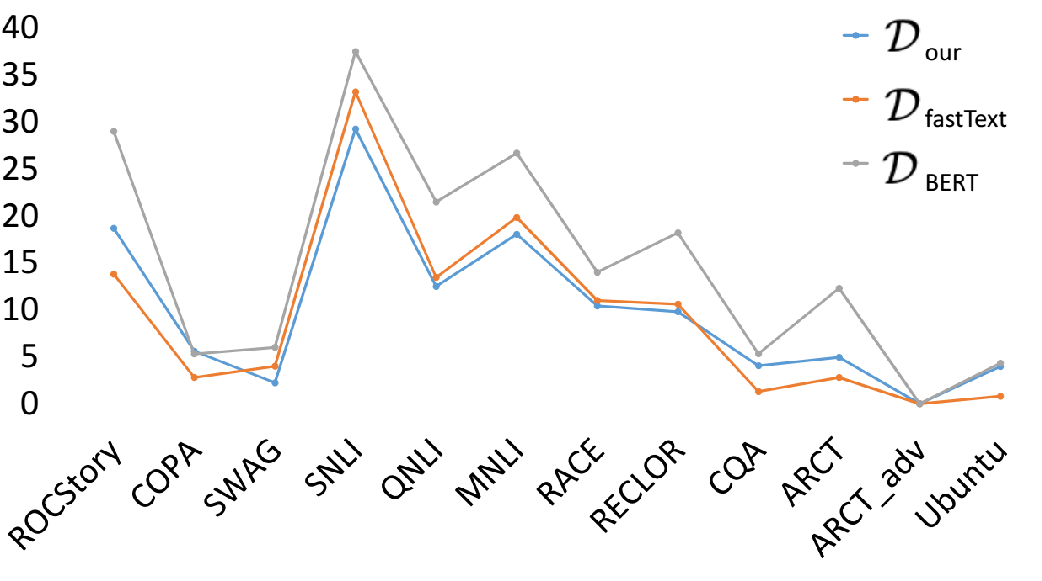
\includegraphics[width=0.7\columnwidth]{picture/d_figure.pdf}
%\caption{Deviation scores for three prediction models on all 12 datasets. 
%``Our'' means our logistic regression model.}
%\label{fig:d_figure}
%\end{figure}

%of $w$ with respect to label $l$ as
%%\KZ{Consider changing $\mathcal{F}$ to $\mathcal{B}$ to avoid confusion with $f$?}
%
%\begin{equation}
%    f_{\mathcal{F}}^{l} = f_{\mathcal{F}}(w, l),    
%\end{equation}
%%We call $f_{\mathcal{F}}^{(k,l)}$ \textit{cue metric}, 
%where $f_{\mathcal{F}}^{l}$ is a function which measures how much spurious information can be conveyed by token $w_k$ for a particular label $l$. 
%$\mathcal{F}$ is a set of cue metrics that we used for computing the \textit{cue score}. 

\subsubsection{Sentiment}

We assign sentiment features as 
positive, negative, or neutral to each hypothesis $h$: 
$sentiment(h) = \sgn(\mbox{num of positive words} - \mbox{num of negative words})$.
%in the hypothesis.
The sentiment polarity of a word
is determined by a look-up from pre-trained
sentiment lexica\footnote{NLTK: \url{https://www.nltk.org}}. 

\subsubsection{Tense}

Considering that the temporal order of events can be also 
important information for inference tasks, we include 
\textit{past}, \textit{present}, \textit{future} as Tense features. 
The tense is determined by verb tags after POS tagging.

\subsubsection{Negation}

Much work has observed that strongly negative words (``no'', ``not'') 
cause the model to predict contradiction for
neutral or entailed statements. Thus we think negation feature can be a factor which affects models in decision-making. 
Negation is decided by dependency parsing~\footnote{Scipy: \url{https://www.scipy.org}}.

\subsubsection{Overlap}
In many cases, substantial word-overlap between the premise and the
hypothesis sentences causes wrong entailment prediction, 
even if they are unrelated. 
%Very little word overlap causes a prediction
%of neutral instead of entailment. 
Thus we wonder 
whether overlap feature really influences models. 
We filter stop words, for example ``a'' and ``the'', before investigating overlap feature. 


\subsubsection{NER}
%\KZ{Rephrase this: The failure for the NER tests in CheckList
%indicates that these models are relying on shortcuts.}
Checklist constructs some stress tests for some NER features. The performance 
of models dropped heavily which indicates that these models are not robust and may 
take advantage of shortcuts.
For example, some name like ``Tom'' mostly appears with label ``contradiction'' 
may influence the decision of models.
%For example anchoring on named entities too strongly
%instead of understanding the reasoning behavior. 
We take NER features, like \textit{location}, \textit{person}, \textit{orgnization}, in our feature test.

\subsubsection{Typos}
The premise or the hypothesis is ill-formed because of spelling errors. 
Typo feature may also be learned by models as off-site information. 
We use a pretrained spelling model~\footnote{\url{https://github.com/barrust/pyspellchecker}} 
to detect the typos in a sentence. 

%We only pay attention to the features which have enough test data for model evaluation.
%In addition, we can analysis the credibility of test data through 
%the Kullback-Leibler (KL) Divergence. If a train dataset distribution is unbalance, 
%a similar distribution between train and T
%test can lead to insufficient test which test the cues mostly with a certain label. 

%\subsection{Data Set Filter}
%\label{sec:generate}
%Given the features $F$, 

%distribution and red distribution represent  the training and test data 
%distribution on the predication values respectively.  
%We use mean square error (MSE) to measure the balance 
%of a feature in a dataset. If the filtered training data distribution is 
%unbalanced on a feature, this feature can be seen as bias.  
%If this bias also exists in test data, indicating 
%a similar distribution exists in the test data, 
%this feature is considered a cue. 

%We show the distribution of some filtered SNLI datasets 
%in~\figref{fig:dataset_result}. 
%We can see that Word feature ``speaking'' mostly correlates with 
%label ``entailment''. So ``speaking'' is a bias. 
%The similar shape between the training and test data distribution indicates 
%this bias is a cue. Low Jensen-Shannon Divergence (JSD) score between the two
%distributions re-affirms our conclusion. 
%Compared with ``speaking'', Word feature ``pushing'' has lower MSE 
%score, but is still much higher than average distribution.  
%Thus ``pushing'' is also a bias. However we can observe that there is little similarity between 
%the train and test distribution. Therefore ``pushing'' is not a cue.
%With filtering and visualizing, we can analysis the biases 
%and cues in datasets. 
%Biases can influence models and cues make the evaluation unauthentic. 

%\begin{figure}[th]
%\centering
%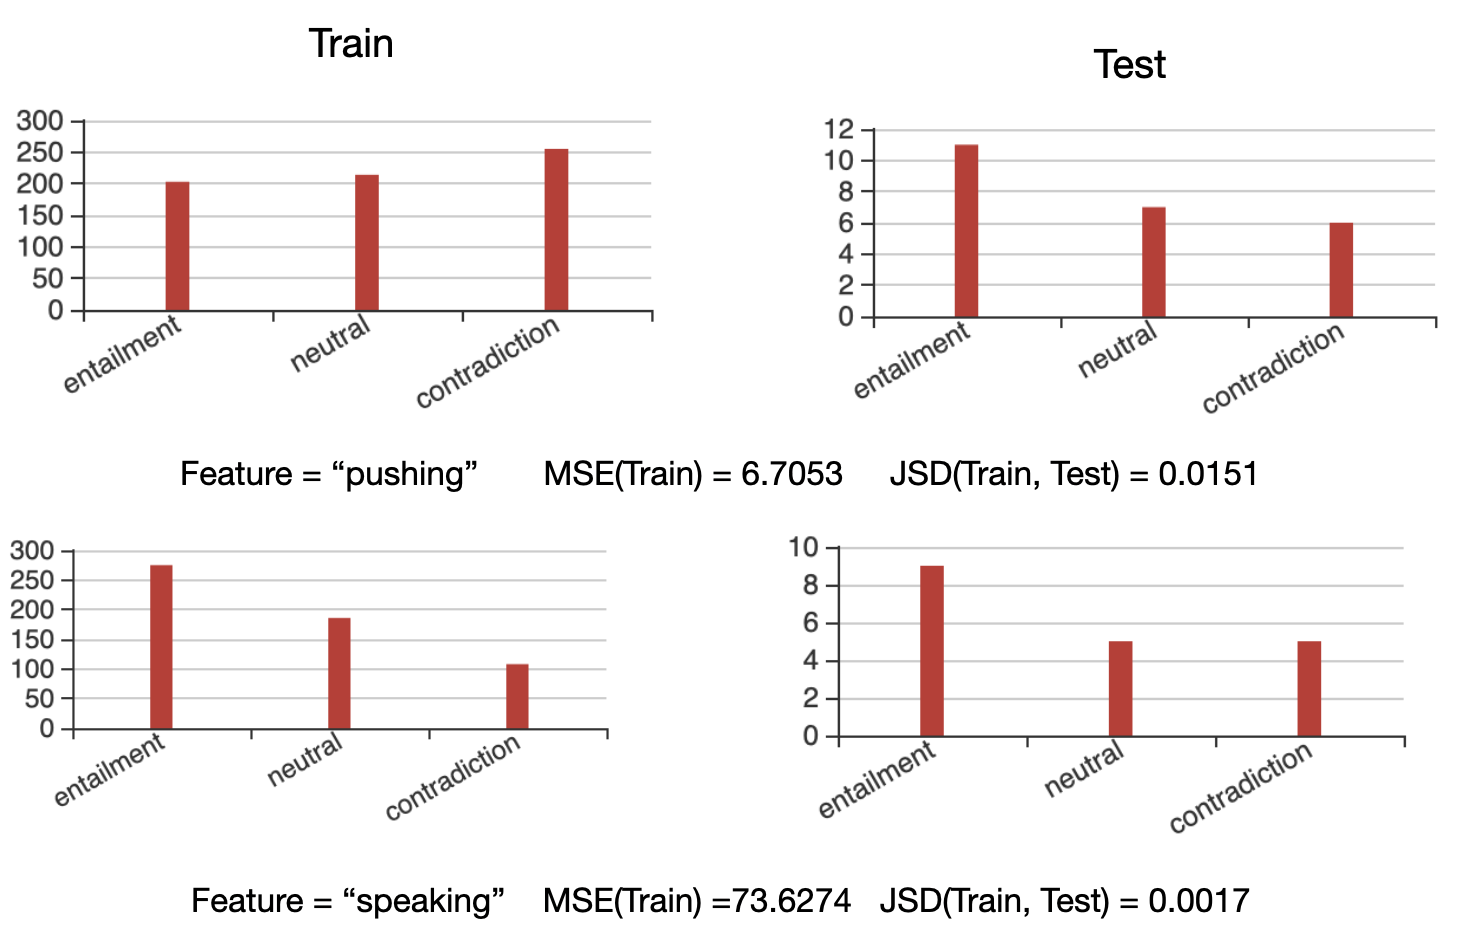
\includegraphics[width=1.0\columnwidth]{picture/dataset_result.jpg}
%\caption{Two examples of dataset distribution on features.}
%\label{fig:dataset_result}
%\end{figure}

\subsection{Model Evaluation}
\label{sec:model}

%We filter cases with specific features $F$ from the training and test data. 
For a specific feature, we filter the examples related to this feature from training and test dataset in~\figref{fig:framework}. 
For example, if we concern about ``Negation'' feature, we will extract all samples which contain negation tags on its parse tree. We can get feature distribution of filtered training data based on each label which is used as a reference for the model prediction distribution. The filtered test data is used to generate stress test that will be introduced in the following. 
In this filtering process, we don't retrain the model or change 
the parameters of models.

%Similar to discovering biases and cues, 
For investigating the bias of models, we can probe models by  
comparing the distribution of the model prediction results and 
the training data. We use JSD here to represent the deviation. 
The smaller the value of JSD, the more the model is affected 
by the distribution of training data.
%but don't provide new method for data augmentation. 
%We require a more fair dataset to test if a model is sensitive to a feature. 
The filtered test dataset of a feature in \figref{fig:framework} (red) is unbalanced among 
labels. The number of cases for each label can be denoted as $c_{ent}, c_{neu}, c_{con}$~(in 
SNLI task). If any of these number is smaller than a threshold $\sigma$, 
we won't consider this feature as a cue at all, because
 this feature is not well supported by enough data. 
%If the smallest number of samples among different labels is lower than 
%a threshold $\sigma$, we won't consider to test this feature. Because
% this feature is not well supported by enough data. 
%The smallest number can be denoted as $c_{min}=min(c_{ent}, c_{neu}, c_{con})$.
The maximum number can be denoted as $c_{max}=max(c_{ent}, c_{neu}, c_{con})$.
To make the result more intuitive and fair, 
we flatten the distribution by repeating $c_{max} - c_{l}$ cases from the filtered cases with label $l$ 
resulting in the orange ``stress test'' 
in \figref{fig:framework}. 
Then we test the model on this stress test. 
The similarity between prediction result (green) and 
training data distribution (blue) on a feature indicates how the model 
is influenced by the appearance of this feature in training data. 
For example, in \figref{fig:model_result}, we use 
ESIM~\cite{chen2016enhanced} model on SNLI. 
We can find that the model is affected by some bias features. 
Given ``pushing'', it still prefers to choose \textit{contradiction}. 
Further, it prefers to choose \textit{entailment} or \textit{neutral} with ``speaking''.  
JSD score for these two examples are also very low. 
%With comparison, we can find that models are sensitive to some bias features. 

%It is insufficient for testing if the filtered test data size is quite small or samples on 
%some label is rare which bellow a threshold $\sigma$. 
%Thought we can't generate cases for feature, we can point out what kind of 
%test samples should be augmented. 

\begin{figure}[th]
\centering
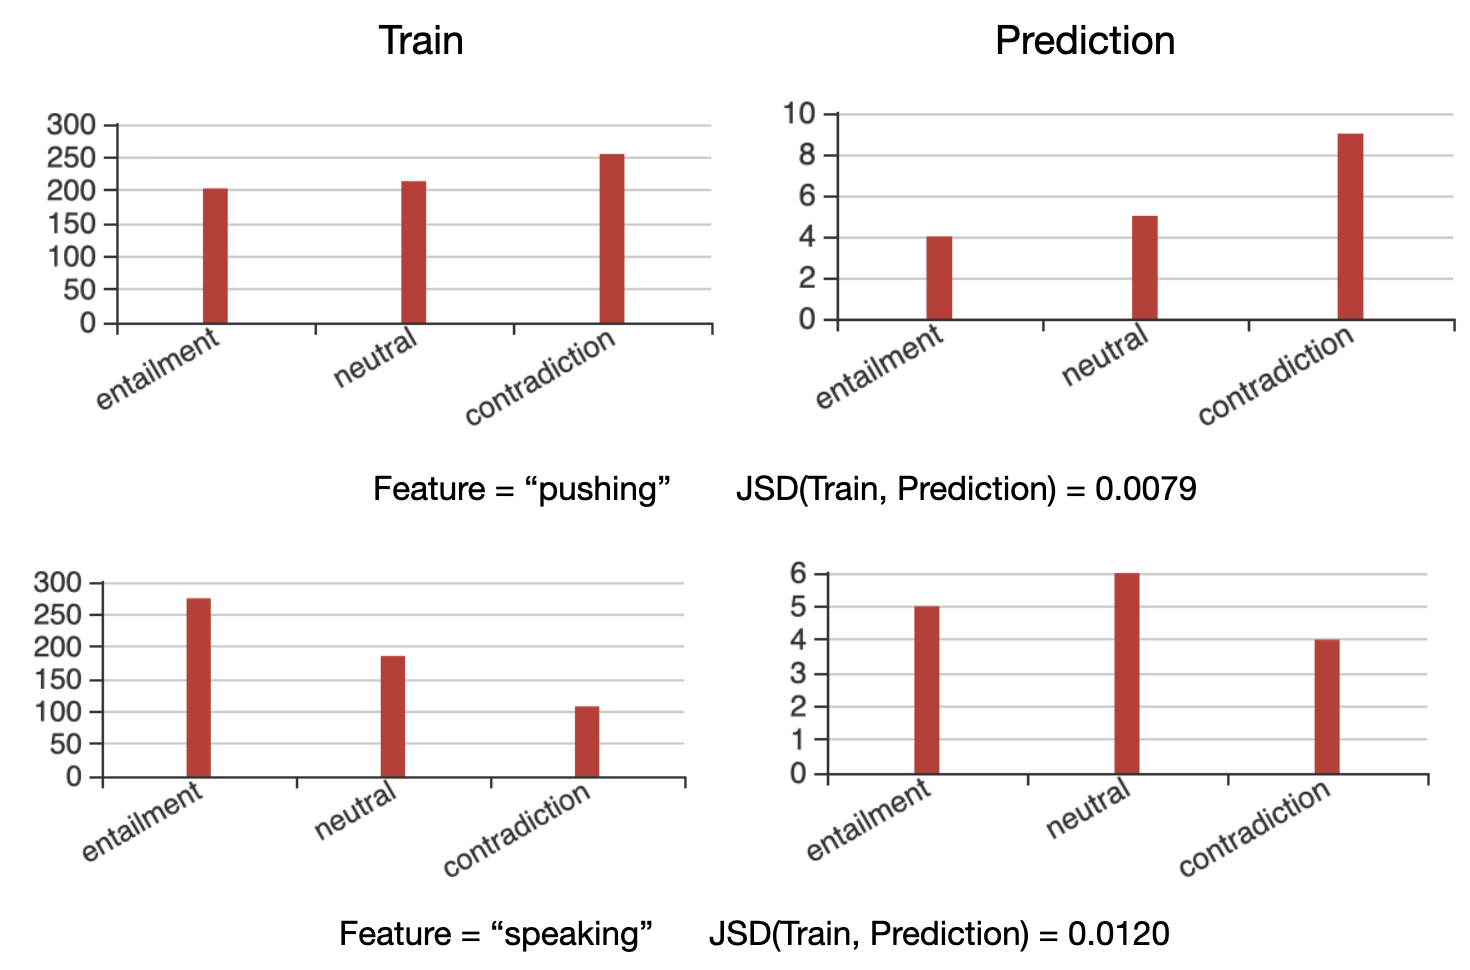
\includegraphics[width=1.0\columnwidth]{picture/model_result.jpg}
\caption{Two examples of model prediction result distribution on features.}
\label{fig:model_result}
\end{figure}


%The similarity is 
%calculated by Kullback-Leibler (KL) Divergence.

\section{CDMiner Demonstration}
\label{sec:demo}

\begin{figure*}[th]
\centering
\includegraphics[width=2\columnwidth]{img/final.eps}
\caption{Result Page for ``dragon'' from CDminer}
\label{fig:demo}
\end{figure*}


We demonstrate CDMiner by building an online search engine\footnote{\url{http://adapt.seiee.sjtu.edu.cn/cdminer}} that can measure and visualize culture
differences between equivalent terms in English and Chinese. We use cosine-knn method,
which achieves the best performance in evaluation part,
as our background technique to support CDMiner.

The front page shows a search box, a cultural difference scale,
a series of sample pictures and
two nearest neighbors graphs from English and Chinese cultures.
User can enter either an English or a Chinese term in 
the search box. 
\figref{fig:demo} shows the result page returned by 
searching ``dragon''.
%CDMiner will direct to the corresponding page.
Below the search box, 
CDMiner shows a spectrum that indicates where the search term stands
among all terms by the amount of cultural difference it has between
English and Chinese.
CDMiner also gives top 4 English and Chinese pictures according to Bing image search.
 In order to get a better view,
``More'' button links to the Bing image search to show you more pictures.
The nearest neighbors lists top 15 related terms in both language 
using a 2-d visualization (\figref{fig:neighbor}). 
Each circle links to the word's own result page.
Meanwhile, the full list of related words is visible when you 
click on ``click to see full list'' button. 

\begin{figure}[ht]
\centering
\includegraphics[width=0.7\columnwidth]{img/en_single.eps}
\caption{Nearest Neighbors Graph for ``dragon''}
\label{fig:neighbor}
\end{figure}



\section{Conclusion}

In this paper, we incorporated the idea of Cookie Theft picture description task into the evaluation of the high-level cognitive abilities of LVLMs and designed a novel evaluation benchmark called CogBench.
% Images in CogBench are of high quality and require more cognitive reasonings to understand, which makes it different from existing image datasets.
The images in CogBench are of high quality and demand more complex cognitive reasoning for interpretation, setting it apart from existing image datasets.
% It consists of a image description task and a VQA task.
Experiments show that there is still a large gap between the cognitive abilities of LVLMs and human beings, indicating CogBench is a challenging benchmark.

% In the future


%\section*{References}


%\begin{thebibliography}{00}
\bibliographystyle{IEEEtran}

\bibliography{IEEEabrv,aaai21}
%\end{thebibliography}


\end{document}
